\documentclass[letter]{IEEEtran}
% Add the compsoc option for Computer Society conferences.
%
% If IEEEtran.cls has not been installed into the LaTeX system files,
% manually specify the path to it like:
% \documentclass[conference]{../sty/IEEEtran}


%
\ifCLASSINFOpdf
   %\usepackage[pdftex]{graphicx}
  % declare the path(s) where your graphic files are
  % \graphicspath{{../pdf/}{../jpeg/}}
  % and their extensions so you won't have to specify these with
  % every instance of \includegraphics
  % \DeclareGraphicsExtensions{.pdf,.jpeg,.png}
\else
  % or other class option (dvipsone, dvipdf, if not using dvips). graphicx
  % will default to the driver specified in the system graphics.cfg if no
  % driver is specified.
  % \usepackage[dvips]{graphicx}
  % declare the path(s) where your graphic files are
  % \graphicspath{{../eps/}}
  % and their extensions so you won't have to specify these with
  % every instance of \includegraphics
  % \DeclareGraphicsExtensions{.eps}
\fi
% graphicx was written by David Carlisle and Sebastian Rahtz. It is
% required if you want graphics, photos, etc. graphicx.sty is already
% installed on most LaTeX systems. The latest version and documentation can
% be obtained at: 
% http://www.ctan.org/tex-archive/macros/latex/required/graphics/
% Another good source of documentation is "Using Imported Graphics in
% LaTeX2e" by Keith Reckdahl which can be found as epslatex.ps or
% epslatex.pdf at: http://www.ctan.org/tex-archive/info/
%
% latex, and pdflatex in dvi mode, support graphics in encapsulated
% postscript (.eps) format. pdflatex in pdf mode supports graphics
% in .pdf, .jpeg, .png and .mps (metapost) formats. Users should ensure
% that all non-photo figures use a vector format (.eps, .pdf, .mps) and
% not a bitmapped formats (.jpeg, .png). IEEE frowns on bitmapped formats
% which can result in "jaggedy"/blurry rendering of lines and letters as
% well as large increases in file sizes.
%
% You can find documentation about the pdfTeX application at:
% http://www.tug.org/applications/pdftex





% *** MATH PACKAGES ***
%
\usepackage[cmex10]{amsmath}
\usepackage{amssymb}
\usepackage{bm} 

% *** ALIGNMENT PACKAGES ***
%
%\usepackage{array}
% Frank Mittelbach's and David Carlisle's array.sty patches and improves
% the standard LaTeX2e array and tabular environments to provide better
% appearance and additional user controls. As the default LaTeX2e table
% generation code is lacking to the point of almost being broken with
% respect to the quality of the end results, all users are strongly
% advised to use an enhanced (at the very least that provided by array.sty)
% set of table tools. array.sty is already installed on most systems. The
% latest version and documentation can be obtained at:
% http://www.ctan.org/tex-archive/macros/latex/required/tools/


%\usepackage{mdwmath}
%\usepackage{mdwtab}
% Also highly recommended is Mark Wooding's extremely powerful MDW tools,
% especially mdwmath.sty and mdwtab.sty which are used to format equations
% and tables, respectively. The MDWtools set is already installed on most
% LaTeX systems. The lastest version and documentation is available at:
% http://www.ctan.org/tex-archive/macros/latex/contrib/mdwtools/


% IEEEtran contains the IEEEeqnarray family of commands that can be used to
% generate multiline equations as well as matrices, tables, etc., of high
% quality.


%\usepackage{eqparbox}
% Also of notable interest is Scott Pakin's eqparbox package for creating
% (automatically sized) equal width boxes - aka "natural width parboxes".
% Available at:
% http://www.ctan.org/tex-archive/macros/latex/contrib/eqparbox/



% *** SUBFIGURE PACKAGES ***
%\usepackage[tight,footnotesize]{subfigure}
% subfigure.sty was written by Steven Douglas Cochran. This package makes it
% easy to put subfigures in your figures. e.g., "Figure 1a and 1b". For IEEE
% work, it is a good idea to load it with the tight package option to reduce
% the amount of white space around the subfigures. subfigure.sty is already
% installed on most LaTeX systems. The latest version and documentation can
% be obtained at:
% http://www.ctan.org/tex-archive/obsolete/macros/latex/contrib/subfigure/
% subfigure.sty has been superceeded by subfig.sty.

\usepackage{graphicx}
\usepackage{float}
% correct bad hyphenation here
\hyphenation{}
\newcommand{\PEP}{\rm{PEP}}
\newcommand{\BER}{\rm{BER}}
\renewcommand{\Re}{\rm Re}
\renewcommand{\Im}{\rm Im}



\begin{document}
%
% paper title
% can use linebreaks \\ within to get better formatting as desired
\title{Modulation Diversity Design in Cooperative Relay-HARQ Network}


% author names and affiliations
% use a multiple column layout for up to three different
% affiliations
\author{
     \IEEEauthorblockN{Wenhao Wu, Hans Mittelmann, and Zhi Ding}
%     \IEEEauthorblockA{
%         School of Electrical and\\Computer Engineering\\
%         Georgia Institute of Technology\\
%         Atlanta, Georgia 30332--0250\\
%         Email: http://www.michaelshell.org/contact.html
%     }
%     \and
%     \IEEEauthorblockN{Homer Simpson}
%     \IEEEauthorblockA{Twentieth Century Fox\\
%         Springfield, USA\\
%         Email: homer@thesimpsons.com
%     }
%     \and
%     \IEEEauthorblockN{James Kirk\\ and Montgomery Scott}
%     \IEEEauthorblockA{Starfleet Academy\\
%         San Francisco, California 96678-2391\\
%         Telephone: (800) 555--1212\\
%         Fax: (888) 555--1212
%     }
}

% conference papers do not typically use \thanks and this command
% is locked out in conference mode. If really needed, such as for
% the acknowledgment of grants, issue a \IEEEoverridecommandlockouts
% after \documentclass

% for over three affiliations, or if they all won't fit within the width
% of the page, use this alternative format:
% 
%\author{\IEEEauthorblockN{Michael Shell\IEEEauthorrefmark{1},
%Homer Simpson\IEEEauthorrefmark{2},
%James Kirk\IEEEauthorrefmark{3}, 
%Montgomery Scott\IEEEauthorrefmark{3} and
%Eldon Tyrell\IEEEauthorrefmark{4}}
%\IEEEauthorblockA{\IEEEauthorrefmark{1}School of Electrical and Computer Engineering\\
%Georgia Institute of Technology,
%Atlanta, Georgia 30332--0250\\ Email: see http://www.michaelshell.org/contact.html}
%\IEEEauthorblockA{\IEEEauthorrefmark{2}Twentieth Century Fox, Springfield, USA\\
%Email: homer@thesimpsons.com}
%\IEEEauthorblockA{\IEEEauthorrefmark{3}Starfleet Academy, San Francisco, California 96678-2391\\
%Telephone: (800) 555--1212, Fax: (888) 555--1212}
%\IEEEauthorblockA{\IEEEauthorrefmark{4}Tyrell Inc., 123 Replicant Street, Los Angeles, California 90210--4321}}




% use for special paper notices
%\IEEEspecialpapernotice{(Invited Paper)}


% 6 + 1 page policy for globecom

% make the title area
\maketitle


\begin{abstract}
    %\boldmath
    % (what we do)
Modulation diversity (MoDiv) is a practically useful diversity enhancement
technique that utilizes different modulation mappings from bits to constellation
symbols. This approach is particularly effective in hybrid-ARQ (HARQ) systems.
In this paper, we study the optimization of MoDiv in a coordinated relay-HARQ
network to reduce the bit error rate (BER).
    % (how they do)
    % (how we do)
We formulate the MoDiv design optimization problem into a quadratic
three-dimensional assignment problem (Q3AP) solved with a modified iterated
local search (ILS) method. Numerical results demonstrate its performance gain,
and show that when the channels are heavily fading, a comparable BER reduction
is achieved with a heuristic MoDiv scheme.
    % (main results)
\end{abstract}
% IEEEtran.cls defaults to using nonbold math in the Abstract.
% This preserves the distinction between vectors and scalars. However,
% if the conference you are submitting to favors bold math in the abstract,
% then you can use LaTeX's standard command \boldmath at the very start
% of the abstract to achieve this. Many IEEE journals/conferences frown on
% math in the abstract anyway.

% no keywords

% For peer review papers, you can put extra information on the cover
% page as needed:
% \ifCLASSOPTIONpeerreview
% \begin{center} \bfseries EDICS Category: 3-BBND \end{center}
% \fi
%
% For peerreview papers, this IEEEtran command inserts a page break and
% creates the second title. It will be ignored for other modes.
\IEEEpeerreviewmaketitle

%\baselineskip=11pt

\section{Introduction}
% Why are we interested in the cooperative relay-HARQ channel? Why MoDiv?
In modern wireless communication, high rate data transmission often leads
to reception errors. To overcome packet loss due to transmission errors, 
Automatic Repeat reQuest (ARQ) or Hybrid ARQ (HARQ) are important mechanism for
better reliability. HARQ in conjunction with relay networks has attracted great
deal of research interest in recent years~\cite{ngo2014hybrid}. Because symbols
transmitted in practice often utilize linear modulations of finite-size
constellation (e.g., Q-ary PSK, or Q-ary QAM), the performance of cooperative
relay-HARQ systems can benefit from Modulation Diversity 
(MoDiv)~\cite{benelli1992new}, in which each
group of $\log_2 Q$ bits are mapped to different constellation points across
different links and in different transmissions. 

There is a number of research works on MoDiv for relay
network~\cite{seddik2008trans, khormuji2008rate} and relay-HARQ
system~\cite{kim2009design, ryu2011ber, yu2012power}. Despite the encouraging
performance gain, the afore-mentioned works all assume a low bandwidth
efficiency scheme where (re)transmissions on the Source-Destination (S-D) link
and the Relay-Destination (R-D) links occupy orthogonal bands or time slots.
From this point of view, we study the MoDiv design in a relay-HARQ networks in
Fig.~\ref{fig:system_model} where the S-D and R-D links are coordinatedly additive as in
\cite{cover1979capacity, nabar2004fading,azarian2005achievable}, practically
forming a 2-by-1 multiple-input single-output (MISO) diversity system. In this
context, we formulate the bit error rate (BER) minimization MoDiv design into a
quadratic three-dimensional assignment problem (Q3AP). Though Q3AP is NP-hard so
that the MoDiv design problem can not be solved exactly in practice even for a
middle size constellation such as 16-QAM, there are a number of heuristic
algorithms~\cite{drezner2008extensive, james2009multistart,benlic2015memetic}
for its reduced form, Quadratic Assignment Problem (QAP), that results in
high-quality solutions over the QAPLIB dataset~\cite{burkard1997qaplib}. In this
work, we adopt an efficient modified Iterated Local Search (ILS) method to solve
the Q3AP formulated from BER-minimization MoDiv design problem. Our numerical
results demonstrate significant BER reduction over non-MoDiv HARQ schemes.
Moreover, we also show that when the channels are heavily fading, a comparable
performance gain is offered by an effortless heuristic MoDiv scheme.

\begin{figure}[!t]
    \begin{minipage}[b]{0.48\linewidth}
      \centering
      \centerline{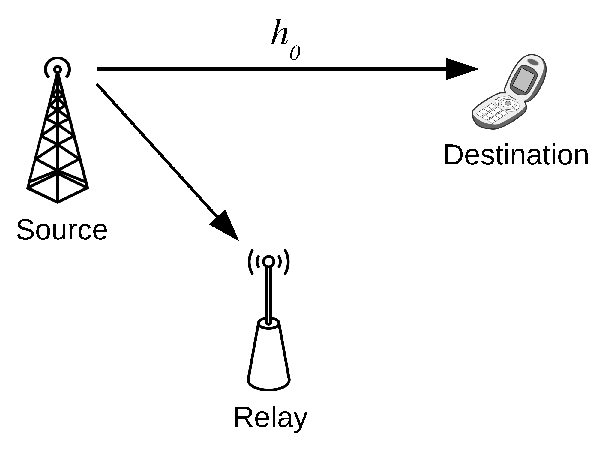
\includegraphics[width=4.0cm]{./figs/relayHARQ1.eps}}
      \centerline{(a) Phase 1}\medskip
    \end{minipage}
    \hfill
    \begin{minipage}[b]{.48\linewidth}
      \centering
      \centerline{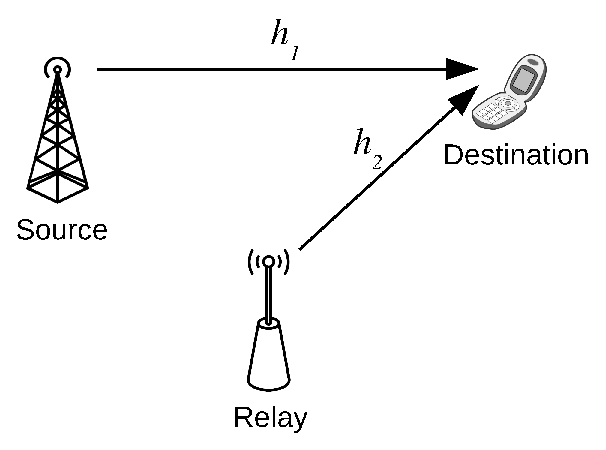
\includegraphics[width=4.0cm]{./figs/relayHARQ2.eps}}
      \centerline{(b) Phase 2}\medskip
    \end{minipage}
    \caption{Cooperative relay-HARQ networks.}
    \label{fig:system_model}
\end{figure}


%\hfill mds

\section{System Model}
\label{sec:model}
% Cooperative relay-HARQ channel 
We consider the cooperative relay-HARQ network shown in
Fig.~\ref{fig:system_model}. There are two phases in this transmission system.
In phase 1, source node broadcasts its packet that can be received by both the
destination and the relay. In phase 2 of this HARQ setup, upon packet loss,
both the relay and the source node cooperatively retransmit the lost packet
information to the destination. Our goal is to design the H-ARQ constellation
mapping for modulation diversity such that the packet BER at the receiver is
minimized.

Denote $\mathcal{C}$ as the constellation used by this relay network whose size
is $Q = |\mathcal{C}|$. In the first phase, the source converts a bit sequence
of length $\log_2Q$ into symbols with Gray mapping $\psi_0: \{0,\ldots,Q -
1\}\rightarrow \mathcal{C}$. The bit sequence is indexed by its decimal
equivalence $p\in \{0,\ldots,Q - 1\}$. The source transmits $\psi_0[p]$ to the
destination via channel $h_0$ which is also overheard by the decode-and-forward
(DF) relay. We assume that this relay is placed strategically such that it has
negligible decoding error rate as in~\cite{ryu2011ber, kim2009design}. Upon
receiving a request for retransmission, the second phase begins with
the source and the relay remapping $p$ into $\psi_1[p]$ and $\psi_2[p]$,
respectively.  In general,  $\psi_1\not=\psi_0$ and $\psi_2\not=\psi_0$. The
remapped symbols are transmitted simultaneously on the same frequency band to the
destination via channels $h_1$ and $h_2$. In summary, the received signals at the
destination during the two phases are, respectively, 
\begin{subequations}
    \begin{align}
       y_1 & = h_0\psi_0[p] + v_1, \\
       y_2 & = h_1\psi_1[p] + h_2\psi_2[p] + v_2,
    \end{align}
\end{subequations}
where $v_1, v_2\sim\mathcal{CN}(0,\sigma_v^2)$ are additive channel noises.
Throughout this work, we assume the channels $h_0$, $h_1$ and $h_2$ follows
independent Rician distribution.

% ML demodulator
Assuming that the destination has perfect channel state information (CSI). Based
on the received symbols $y_1$ and $y_2$,  the destination decodes the data by
identifying the index $p$ via maximum likelihood (ML) detection:
\begin{align}
    \min_{\hat{p}} |y_1 - h_0\psi_0[\hat{p}]|^2 + |y_2-
    h_1\psi_1[\hat{p}] - h_2\psi_2[\hat{p}]|^2.
    \label{eq:ML}
\end{align}

% An example of a floating figure using the graphicx package.
% Note that \label must occur AFTER (or within) \caption.
% For figures, \caption should occur after the \includegraphics.
% Note that IEEEtran v1.7 and later has special internal code that
% is designed to preserve the operation of \label within \caption
% even when the captionsoff option is in effect. However, because
% of issues like this, it may be the safest practice to put all your
% \label just after \caption rather than within \caption{}.
%
% Reminder: the "draftcls" or "draftclsnofoot", not "draft", class
% option should be used if it is desired that the figures are to be
% displayed while in draft mode.
%
%\begin{figure}[!t]
%\centering
%\includegraphics[width=2.5in]{myfigure}
% where an .eps filename suffix will be assumed under latex, 
% and a .pdf suffix will be assumed for pdflatex; or what has been declared
% via \DeclareGraphicsExtensions.
%\caption{Simulation Results}
%\label{fig_sim}
%\end{figure}

% Note that IEEE typically puts floats only at the top, even when this
% results in a large percentage of a column being occupied by floats.


% An example of a double column floating figure using two subfigures.
% (The subfig.sty package must be loaded for this to work.)
% The subfigure \label commands are set within each subfloat command, the
% \label for the overall figure must come after \caption.
% \hfil must be used as a separator to get equal spacing.
% The subfigure.sty package works much the same way, except \subfigure is
% used instead of \subfloat.
%
%\begin{figure*}[!t]
%\centerline{\subfloat[Case I]\includegraphics[width=2.5in]{subfigcase1}%
%\label{fig_first_case}}
%\hfil
%\subfloat[Case II]{\includegraphics[width=2.5in]{subfigcase2}%
%\label{fig_second_case}}}
%\caption{Simulation results}
%\label{fig_sim}
%\end{figure*}
%
% Note that often IEEE papers with subfigures do not employ subfigure
% captions (using the optional argument to \subfloat), but instead will
% reference/describe all of them (a), (b), etc., within the main caption.


% An example of a floating table. Note that, for IEEE style tables, the 
% \caption command should come BEFORE the table. Table text will default to
% \footnotesize as IEEE normally uses this smaller font for tables.
% The \label must come after \caption as always.
%
%\begin{table}[!t]
%% increase table row spacing, adjust to taste
%\renewcommand{\arraystretch}{1.3}
% if using array.sty, it might be a good idea to tweak the value of
% \extrarowheight as needed to properly center the text within the cells
%\caption{An Example of a Table}
%\label{table_example}
%\centering
%% Some packages, such as MDW tools, offer better commands for making tables
%% than the plain LaTeX2e tabular which is used here.
%\begin{tabular}{|c||c|}
%\hline
%One & Two\\
%\hline
%Three & Four\\
%\hline
%\end{tabular}
%\end{table}


% Note that IEEE does not put floats in the very first column - or typically
% anywhere on the first page for that matter. Also, in-text middle ("here")
% positioning is not used. Most IEEE journals/conferences use top floats
% exclusively. Note that, LaTeX2e, unlike IEEE journals/conferences, places
% footnotes above bottom floats. This can be corrected via the \fnbelowfloat
% command of the stfloats package.

\section{Optimal Constellation Mapping for Modulation Diversity}
\label{sec:core}
In this section we first formulate the minimum BER design of MoDiv into a Q3AP problem.
We then elaborate on the numerical approach for computing the input cost matrix of the Q3AP
problem. We then provide an efficient algorithm to obtain the Q3AP solution.

\subsection{BER Minimization via Q3AP solution}
% Q3AP formulation 
Assume that the information-bearing index $p$ follows a uniform distribution,
the BER can be upper-bounded and approximated using the pair-wise error
probability (PEP)~\cite{harvind2005symbol}
\begin{align}
    P_{\BER} \approx \sum_{p=0}^{Q - 1}\sum_{q=0}^{Q - 1}\frac{B[p,
    q]}{Q}P_{\PEP}(q | p), \label{eq:P_BER}
\end{align}
where $B[p,q]$ is the Hamming distance between the binary representation of $p$
and $q$ divided by $\log_2Q$ and $P_{\PEP}(q | p)$ is the probability for the ML
decoder to prefer $q$ over $p$ when $p$ is actually transmitted. According to~(\ref{eq:ML}), we have
\begin{align}
    P_{\PEP}(q | p) = P_{h_0,h_1,h_2,v_1,v_2}\{\delta(p,q,\psi_1,\psi_2) < 0\}.
    \label{eq:P_PEP}
\end{align}
In other words, given indices $p, q$ and the remapping scheme $\psi_1$, $\psi_2$, the
probability of the random variable $\delta<0$ being evaluated over the random
variables $h_0,h_1,h_2,v_1,v_2$, and $\delta$ is defined as
\begin{align}
    \delta & = |h_0(\psi_0[p] - \psi_0[q]) + v_1|^2 - |v_1|^2 +\notag\\ 
    &
    |h_1(\psi_1[p] - \psi_1[q])+h_2(\psi_2[p] - \psi_2[q])+v_2|^2 -
    |v_2|^2.
    \label{eq:delta}
\end{align}
In order to formulate the Q3AP problem, we introduce binary variables
\[
x_{pij}= \left\{\begin{array}{ll}
1,& \mbox{if $\psi_1[p] = \psi_0[i]$ and $\psi_2[p] = \psi_0[j]$}\\
 0,& \mbox{otherwise.} \end{array} \right. \]
Denote $\mathbf{x} = \{x_{pij}|\;p,i,j=0,\ldots,Q-1\}$
and constraint set
\begin{align}
    \mathcal{P} & = \left\{\mathbf{x}:\,\sum_{p=0}^{Q-1}x_{pij} = 1,
    x_{pij}\in\{0, 1\}\right\}, \label{eq:constraint_p}
\end{align}
and $\mathcal{I}$ and $\mathcal{J}$ which are defined as
in~(\ref{eq:constraint_p}) by replacing the summation index $p$ with $i$ and
$j$, respectively. Then from~(\ref{eq:P_BER})(\ref{eq:P_PEP})(\ref{eq:delta}),
the BER minimization MoDiv scheme $\min_{\psi_1, \psi_2}P_{\BER}$ can be
reformulated as
\begin{align}
    & \min_{\mathbf{x}}\sum_{p=0}^{Q-1}\sum_{i=0}^{Q-1}\sum_{j=0}^{Q-1}
    \sum_{q=0}^{Q-1}\sum_{k=0}^{Q-1}\sum_{l=0}^{Q-1}c_{pijqkl}x_{pij}x_{qkl},
    \label{eq:Q3AP}\\
    & \mbox{s.t. } \mathbf{x}\in \mathcal{P}\cap\mathcal{I}\cap\mathcal{J}.
    \notag
\end{align}
in which
\begin{align}
    c_{pijqkl} & = \frac{B[p, q]}{Q}P_{h_0,h_1,h_2,v_1,v_2}\{\delta(p,i,j,q,k,l)
    < 0\},
    \label{eq:cpijqkl} \\
    \delta & = |h_1(\psi_0[i] - \psi_0[k])+h_2(\psi_0[j] - \psi_0[l])+v_2|^2 
 \notag
    \\
    &
       + |h_0(\psi_0[p] - \psi_0[q]) + v_1|^2 - |v_1|^2 -
    |v_2|^2.\label{eq:delta_pijqkl}
\end{align}

\subsection{Computation of the Pair-wise Symbol Error Rate}

% serial expansion method
In this section we focus on the computation of the parameters $\{c_{pijqkl}\}$
of the Q3AP problem. According to~(\ref{eq:cpijqkl}), the key to compute
$c_{pijqkl}$ lies in the evaluation of
$P_{h_0,h_1,h_2,v_1,v_2}\{\delta(p,i,j,q,k,l)$, i.e. the cumulative distribution
function (CDF) of the random variable $\delta(p,i,j,q,k,l)$ as
in~(\ref{eq:delta}).Define the moment generating function (MGF)
\[\Phi_{\delta}(\omega) = \mathbb{E}_{\delta}[\exp(-\omega\delta)].\]
Under the well known Rician channel model, 
$h_m\sim\mathcal{CN}(\mu_{h_m},\sigma_{h_m}^2), m=0,1,2$, we 
can extend the method
in~\cite{harvind2005symbol, taricco2002exact} to compute
$P_{h_0,h_1,h_2,v_1,v_2}\{\delta(p,i,j,q,k,l) < 0\}$:
\begin{align}
    & P_{h_0,h_1,h_2,v_1,v_2}\{\delta(p,i,j,q,k,l) < 0\} \notag \\
    & \approx \frac{1}{2v}\sum_{t=1}^v \Re\left\{\Phi_{\delta}(\xi +
    j\xi\tau_t)\right\} + \tau_t\Im\left\{\Phi_{\delta}(\xi +
    j\xi\tau_t)\right\},
    \label{eq:expansion}
\end{align}
where $\tau_t = \tan((t- 1/2)\pi/v)$
and $\Re\{\cdot\}$, $\Im\{\cdot\}$ denote the real and image parts,
respectively. 
The parameter $\xi$ is selected to ensure convergence of the
integration and $\xi = 1/4$ was suggested in \cite{taricco2002exact}. The
size $v$ of the expansion~(\ref{eq:expansion}) needs to be large when $
P_{h_0,h_1,h_2,v_1,v_2}\{\delta(p,i,j,q,k,l) < 0\}$ is small in order to
maintain an acceptable numerical accuracy.

To compute $\Phi_{\delta}(\omega)$, denote the Gaussian random vectors
$\mathbf{z}_1 = [h_0, v_1]^T$, $\mathbf{z}_{2} = [h_1, h_2, v_2]^T$, such
that $\mathbf{z}_m\sim\mathcal{CN}(\bm{\mu}_m, \mathbf{\Sigma}_m)$, $m=1,2$,
where
\begin{align}
    \bm{\mu}_1 = [\mu_{h_0}, 0]^T,& \; \bm{\mu}_{2} = [\mu_{h_1}, \mu_{h_2},
    0]^T,
    \\
    \mathbf{\Sigma}_1 = \mbox{diag}\left(\sigma_{h_0}^2, \sigma_v^2\right), & \;
    \mathbf{\Sigma}_2 = \mbox{diag}\left(\sigma_{h_1}^2, \sigma_{h_2}^2,
    \sigma_v^2\right).
\end{align}
Then~(\ref{eq:delta}) can be rewritten as $\delta =
\mathbf{z}_1^H\mathbf{A}_1\mathbf{z}_1 +
\mathbf{z}_{2}^H\mathbf{A}_{2}\mathbf{z}_{2}$, where
\begin{subequations}
    \begin{align}
        \mathbf{A}_1 & = \left[
            \begin{array}{cc}
                |e_{pq}|^2  & e_{pq}^* \\
                e_{pq} & 0
            \end{array}
        \right], \\
        \mathbf{A}_2 & = \left[
            \begin{array}{ccc}
            |e_{ik}|^2 & e_{ik}^*e_{jl} & e_{ik}^*
            \\
            e_{ik}e_{jl}^* & |e_{jl}|^2 & e_{jl}^*
            \\
            e_{ik} & e_{jl} & 0
        \end{array}
        \right],
    \end{align}
\end{subequations}
here $e_{ab} = \psi_0[a] - \psi_0[b]$. Then the MGF
is
\begin{align}
    \Phi_{\delta}(\omega) & = \sum_{m=1,2}
    \frac{\exp(-\omega\bm{\mu}_m^H\mathbf{A}_m(\mathbf{I} +
    \omega\mathbf{\Sigma}_m\mathbf{A}_m)^{-1}\bm{\mu}_m)}{\det(\mathbf{I} +
    \omega\mathbf{\Sigma}_m\mathbf{A}_m)}.
\end{align}

In our simulation, we implement the above procedure for 16-QAM and 32-QAM with
Armadillo library~\cite{sanderson2010armadillo} on a workstation with 48 cores and
finished the computation in several days for a $Q=32$ case and a few hours for a
$16-QAM$ case. For larger constellation such as 64-QAM, however, the time and
spacial complexity may still be too high. We will address in future works to
reduce this complexity by adding a few rules to restrict the remapping schemes.

\subsection{Q3AP Solution}
% Description of the Q3AP solution methods
For practical-sized constellation such as 16-QAM and 32-QAM, it is impractical
to apply the exact branch-and-bound algorithm~\cite{hahn2008quadratic}. Also,
our tests show that they do not have enough symmetry to exploit for faster
solution as does the 16-PSK constellation~\cite{mittelmann2015solving}.
Consequently, the MoDiv problem is solved with the ILS
method~\cite{hahn2008quadratic} extended from its QAP
version~\cite{stutzle2006iterated}. Starting from two random initial mappings
$\psi_1^{(0)}, \psi_2^{(0)}$, the algorithm executes a local search by
attempting to exchange the mapping of exactly 2 indices in order to lower the
objective function and whenever a reduction in the objective function is made
the mapping is updated. When it hits a local minimum, it executes a perturbation
step by exchanging the mapping of $k_p$ indices, where $k_p$ is adaptively
adjusted within $[k_{p,min}, k_{p,max}]$. The perturbation is accepted with a
probability defined as in simulated annealing, after which the local search is
restarted from the new mappings until the stopping criterion is satisfied.

\subsection{A Heuristic MoDiv Scheme}
\label{sec:heuristic}
The MoDiv design problem can be simplified if we force $\psi_1=\psi_2$. Also,
from~(\ref{eq:delta}), a simple heuristic is that the two indices mapped to two
symbols close to each other in Phase 1 should be mapped to two
symbols far apart in Phase 2. A simple remapping scheme based on this heuristic
is given by Seddik in~\cite{seddik2008trans}. We will show in the next section
that when the channels are heavily fading, this heuristic remapping offers
comparable performance gain as our Q3AP-based MoDiv.

\section{Numerical Results}
\label{sec:simulation}
% Simulation settings
In our simulation, all Rician channels are assumed to have the same Rician
parameter $K$. Also we assume that during the second phase, the phases of the
line of sight (LOS) components of channels $h_1$ and $h_2$ can be aligned at the
source and relay, respectively.
Consequently, we define $\mu_{h_0} = \mu_{h_1} = \sqrt{K/(K + 1)}$,
$\mu_{h_2}=a\sqrt{K/(K + 1)}$,  $\sigma_{h_0}^2 = \sigma_{h_1}^2 = 1/(K+1)$ and
$\sigma_{h_2}^2 = |a|^2/(K+1)$, where $a$ represents the ratio
between the amplitude of the LOS component of the
relay-to-destination and the S-D link. Throughout the
simulation we consider 16-QAM constellation, i.e.,  $Q=16$. The noise power is
parameterized with $E_b/N_0$ of the S-D link.

% Example of Q3AP mapping
First, we provide an example of Q3AP optimized MoDiv. When $E_b/N_0 =
2\mbox{dB}$, $K = 10$ and $a = 1$, the remapping scheme of $\psi_0$
(using Gray-mapping), $\psi_1$ and $\psi_2$ is depicted in
Fig.~\ref{fig:example}. For comparison we also plot Seddik's heuristic remapping
$\psi_S$. The results justify the heuristics mentioned in
Section~\ref{sec:heuristic} and both $\psi_1$ and $\psi_2$ are essentially very
close to $\psi_S$. However, we note that in general $\psi_1\not=\psi_2$.

\begin{figure}[!t]
    \begin{minipage}[b]{0.48\linewidth}
      \centering
      \centerline{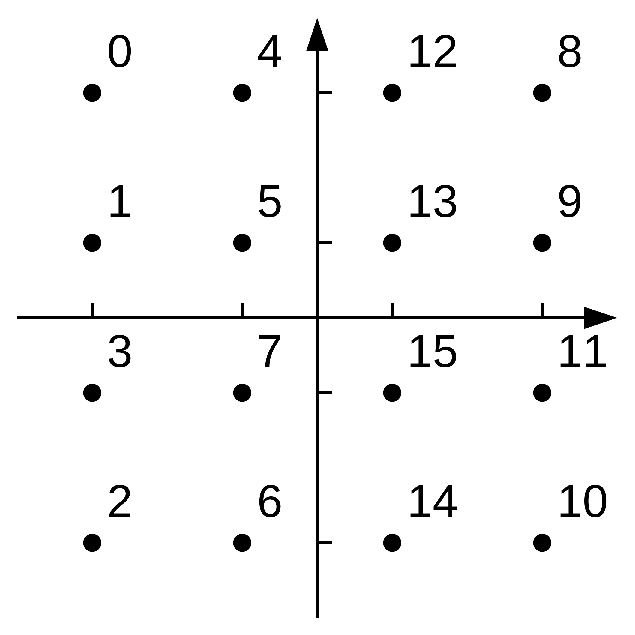
\includegraphics[width=3.0cm]{./figs/gray.eps}}
      \centerline{(a) $\psi_0$ (Gray-mapping)}\medskip
    \end{minipage}
    \hfill
    \begin{minipage}[b]{0.48\linewidth}
      \centering
      \centerline{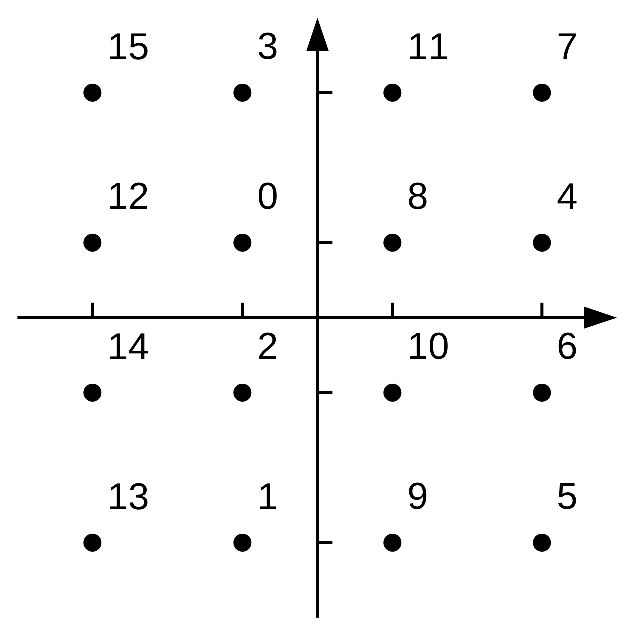
\includegraphics[width=3.0cm]{./figs/karim.eps}}
      \centerline{(b) $\psi_S$}\medskip
    \end{minipage}
    \begin{minipage}[b]{0.48\linewidth}
      \centering
      \centerline{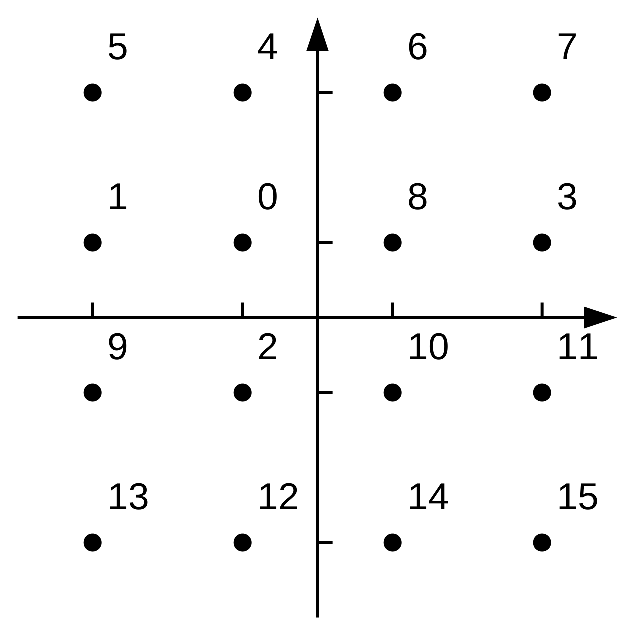
\includegraphics[width=3.0cm]{./figs/psi1.eps}}
      \centerline{(c) $\psi_1$}\medskip
    \end{minipage}
    \hfill
    \begin{minipage}[b]{.48\linewidth}
      \centering
      \centerline{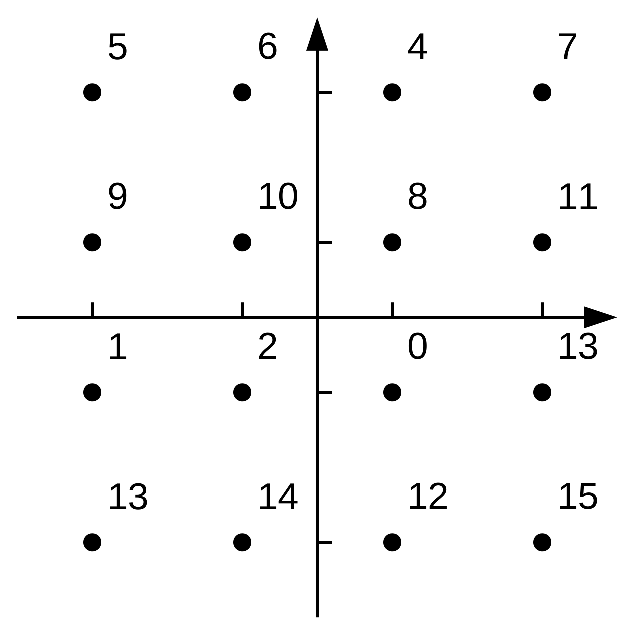
\includegraphics[width=3.0cm]{./figs/psi2.eps}}
      \centerline{(d) $\psi_2$}\medskip
    \end{minipage}
    \caption{Q3AP optimized MoDiv schemes.}
    \label{fig:example}
\end{figure}

% BER Upper bound comparison
Next we compare the BER upper bound $P_{\BER}$, which is also the Q3AP objective
function, for three mapping schemes: the Q3AP optimized MoDiv, the heuristic
MoDiv $\psi_1 = \psi_2 = \psi_S$, and no MoDiv at all, i.e. $\psi_1 = \psi_2 =
\psi_0$. In Fig.~\ref{fig:BERupperbound}, there is a considerable performance
gain for MoDiv versus no MoDiv. Moreover, the gain of the Q3AP optimized MoDiv
over $\psi_1 = \psi_2 = \psi_S$ indicates that different rearrangements at the
source and relay during the cooperative transmission can further boost the BER
performance. However, as $K$ decreases, heuristic MoDiv becomes a good
approximation as the its performance gap with the Q3AP optimized MoDiv
diminishes.

\begin{figure}[!t]
    \begin{minipage}[b]{0.49\linewidth}
      \centering
      \centerline{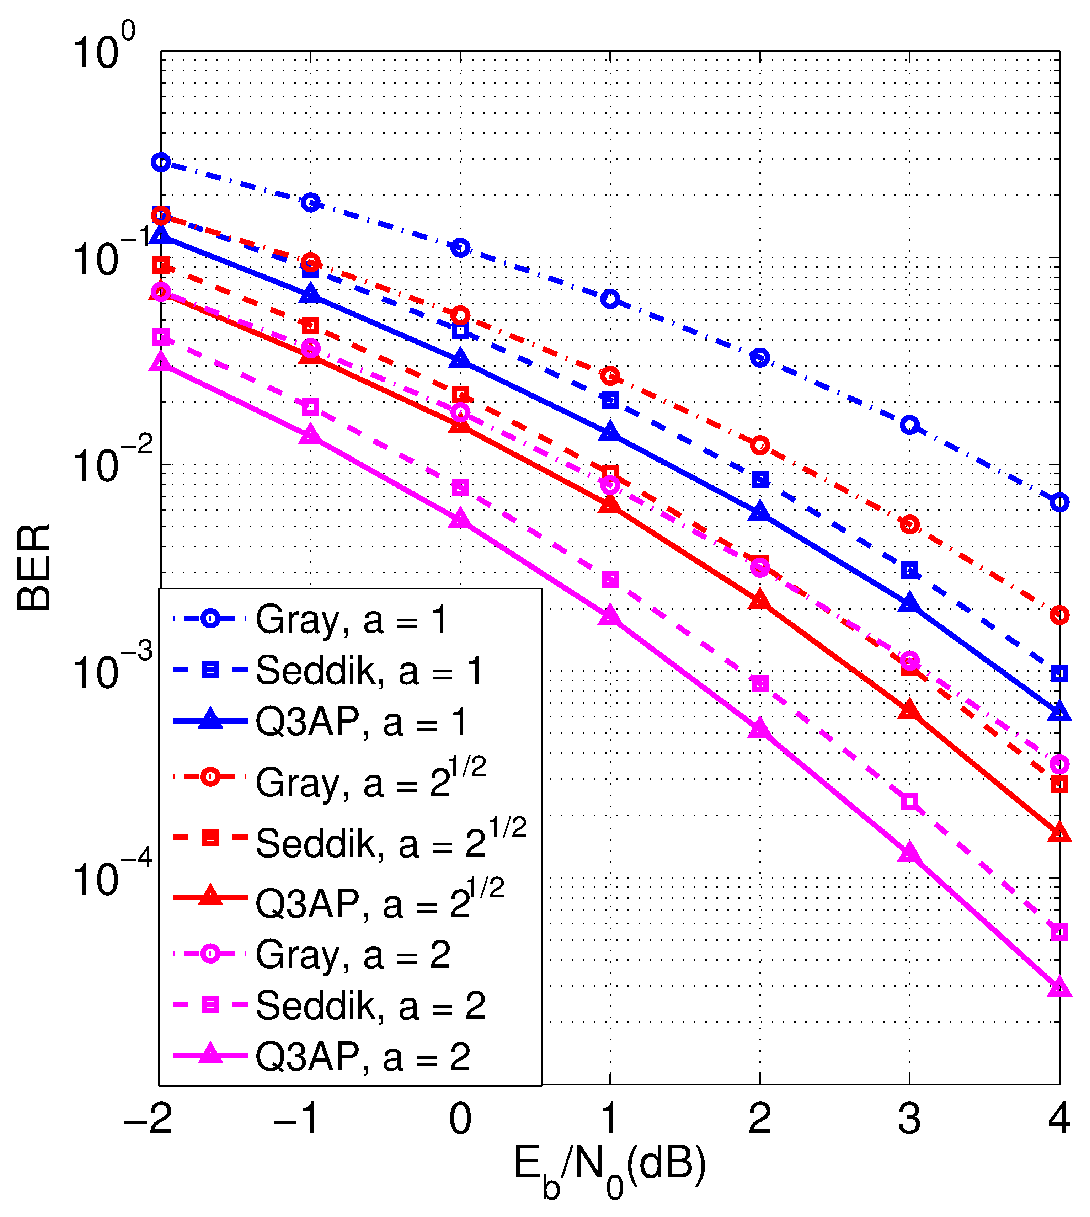
\includegraphics[width=4.2cm]{./figs/bound_10.eps}}
      \centerline{(a) $ K = 10$}\medskip
    \end{minipage}
    \hfill
    \begin{minipage}[b]{0.49\linewidth}
      \centering
      \centerline{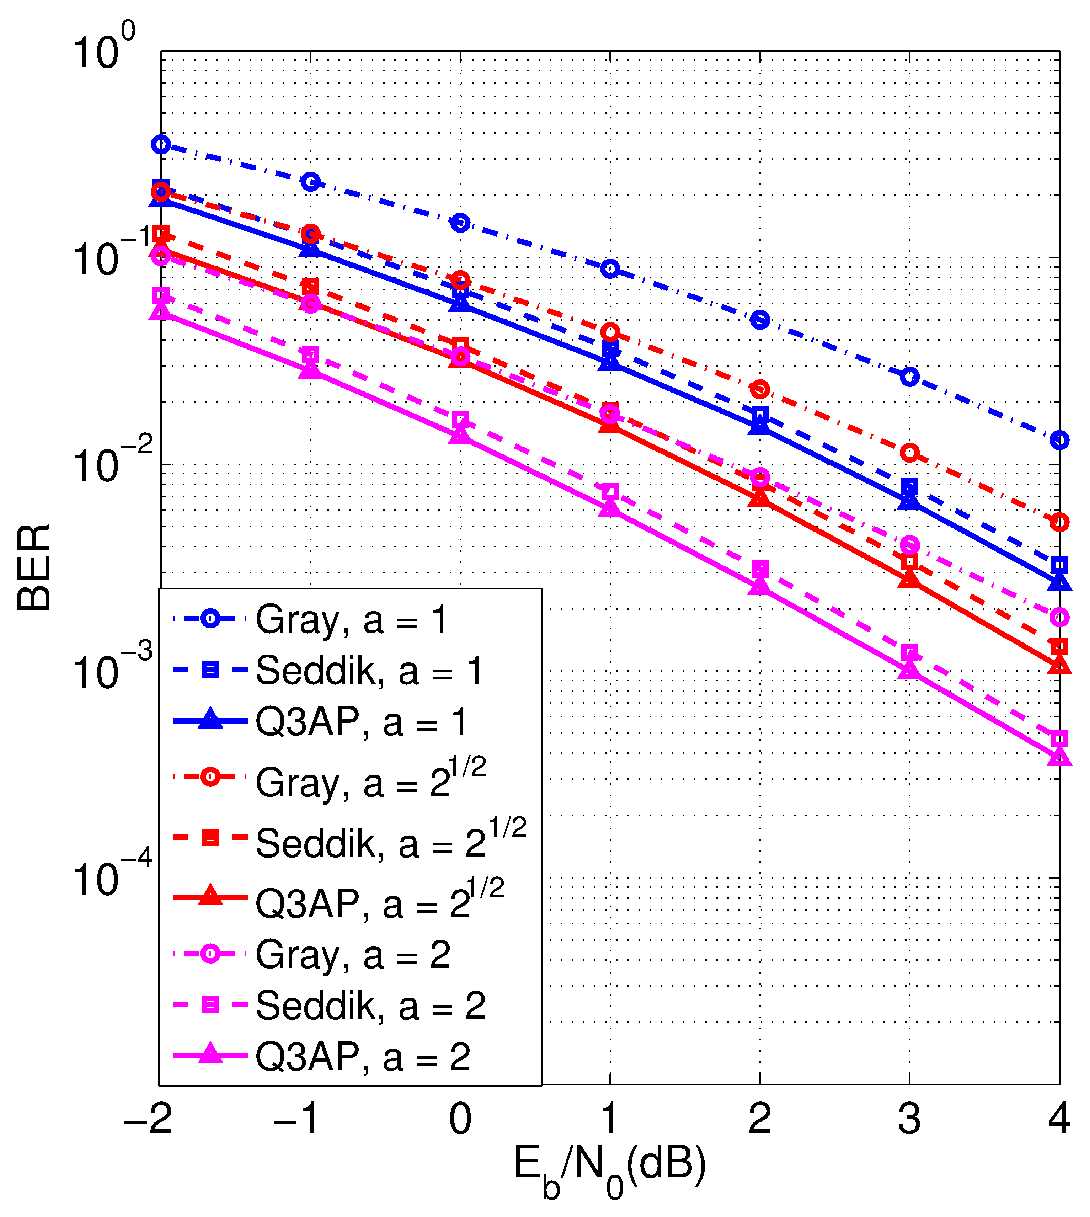
\includegraphics[width=4.2cm]{./figs/bound_5.eps}}
      \centerline{(b) $K=5$}\medskip
    \end{minipage}
    \caption{BER upper bounds of (1) Q3AP optimized MoDiv (2) $\psi_1 = \psi_2 =
    \psi_S$ (3) $\psi_1 = \psi_2 = \psi_0$ for $K = 5, 10$, $a = 1, \sqrt{2},
    2$.}
    \label{fig:BERupperbound}
\end{figure}

% Monte-Carlo BER comparison
The performance gain of MoDiv for the cooperative relay-HARQ
system is further verified with the actual BER evaluated with Monte-Carlo
simulation in Fig.~\ref{fig:montecarlo}. We implement the ML demodulator
in~(\ref{eq:ML}) and evaluate the average BER of $M=10^7$ randomly generated
indices $p$. A similar trend as in Fig.~\ref{fig:BERupperbound} is demonstrated.

\begin{figure}[!t]
    \begin{minipage}[b]{0.49\linewidth}
      \centering
      \centerline{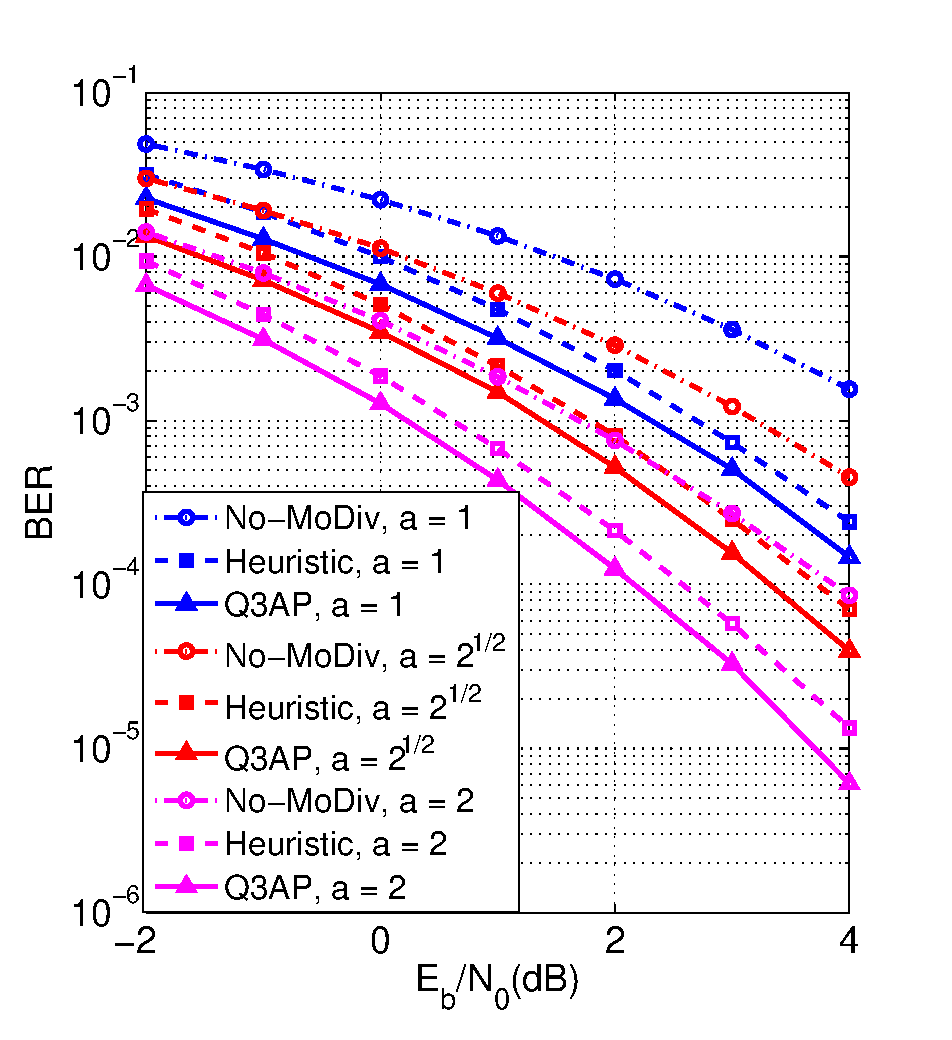
\includegraphics[width=4.2cm]{./figs/MC_10.eps}}
      \centerline{(a) $ K = 10$}\medskip
    \end{minipage}
    \hfill
    \begin{minipage}[b]{0.49\linewidth}
      \centering
      \centerline{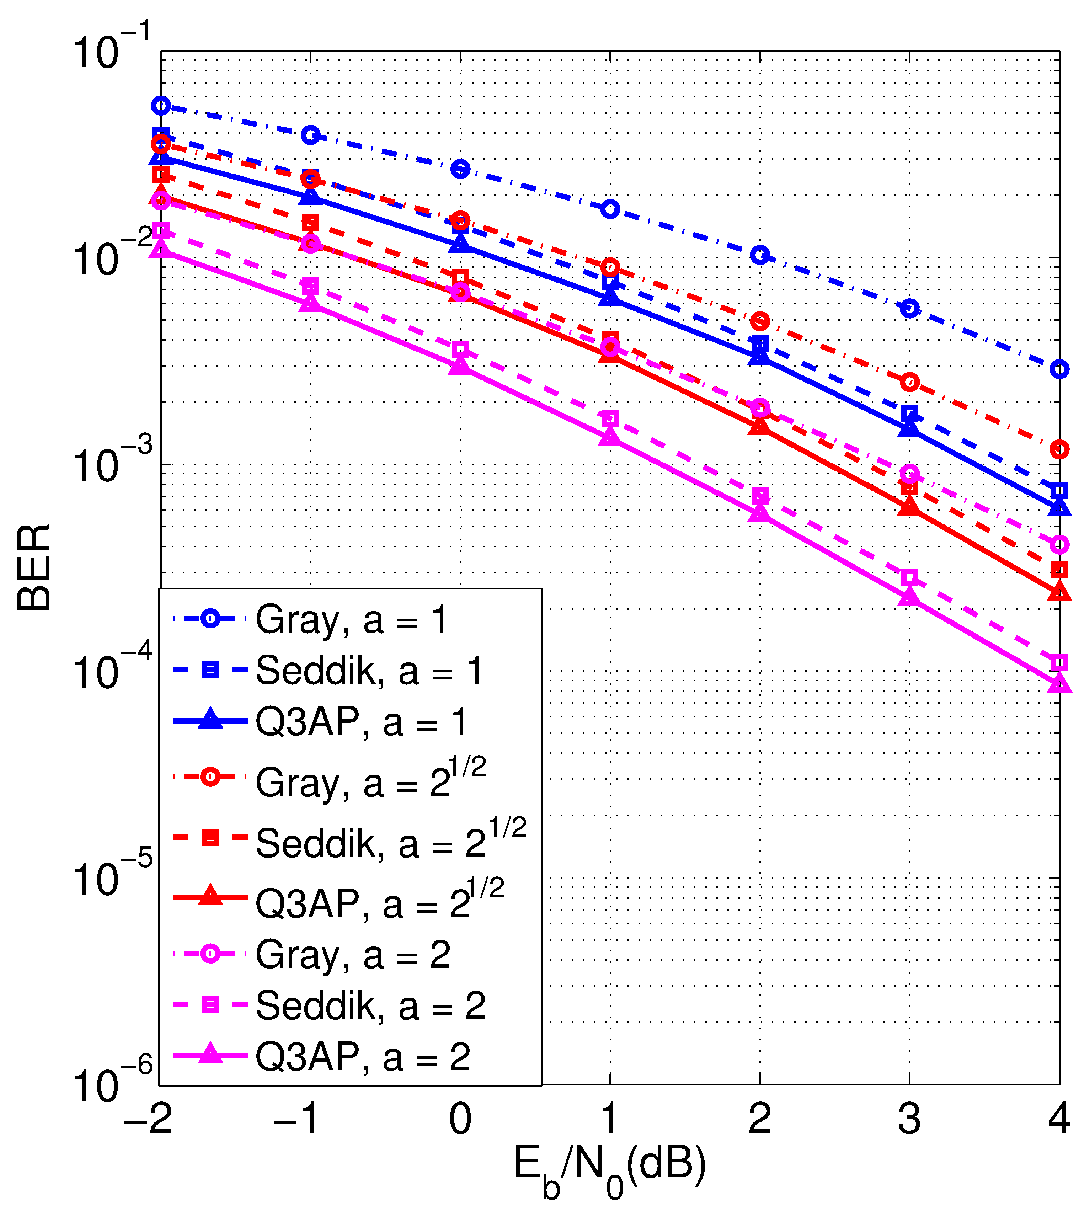
\includegraphics[width=4.2cm]{./figs/MC_5.eps}}
      \centerline{(b) $K=5$}\medskip
    \end{minipage}
    \caption{Monte-Carlo simulated BER of (1) Q3AP optimized MoDiv
    (2) $\psi_1 = \psi_2 = \psi_S$ (3) $\psi_1 = \psi_2 = \psi_0$ for $K = 5,
    10$, $a = 1, \sqrt{2}, 2$.}
    \label{fig:montecarlo}
\end{figure}

% Monte-Carlo BER mismatch comparison
Finally, we test the robustness of the Q3AP MoDiv solution against mismatch in
channel information. The intuition is that in practical systems, the CSI may not
be perfectly accurate and the phase of the LOS component of the S-D and R-D
links may not be perfectly aligned. Also, the Q3AP MoDiv scheme can only be
computed off-line for a limited number of channel settings a priori, instead of
for all possible combinations. We deliberately test the BER performance of the
Q3AP MoDiv solution for channel parameters $a=1$, $K=5$ while the actual channel
setting is $a = \sqrt{2}\exp(j\pi/12)$, $K = 10$. The BER upper bound and
Monte-Carlo simulated BER are plotted in Fig.~\ref{fig:mismatch}. Apparently,
the Q3AP MoDiv solution is not sensitive to the relative amplitude and the phase
alignment error between S-D and R-D links.

\begin{figure}[!t]
    \centering
    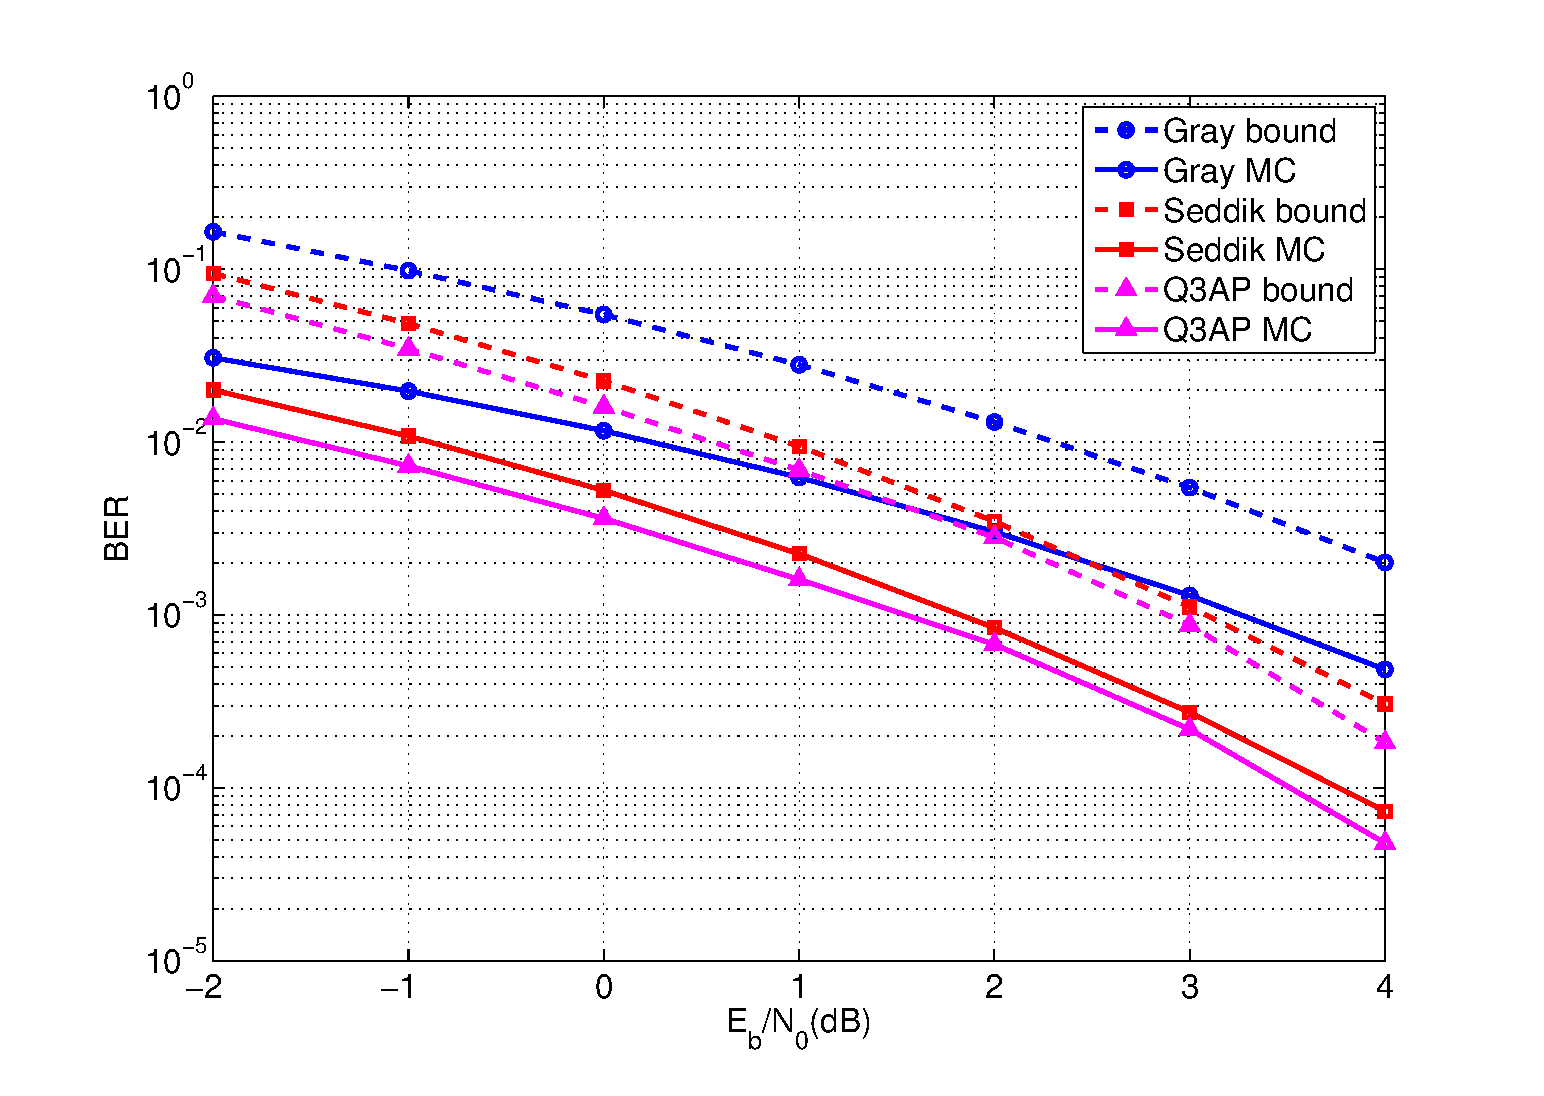
\includegraphics[width=3.0in]{./figs/mismatch.eps}
    \caption{BER performance under channel mismatch. Q3AP MoDiv solution for
    CSI
    $a=1$, $K=5$ while the actual CSIX is $a = \sqrt{2}\exp(j\pi/12)$, $K
    = 10$.}
    \label{fig:mismatch}
\end{figure}

\section{Conclusion}
\label{sec:conclusion}
In this work, we investigated the modulation diversity (MoDiv) design problem in
a three-node cooperative relay-HARQ systems featured by the coordinated
retransmission from both the source and the relay. Aiming to minimize the bit
error rate (BER) upper bound, we formulated the MoDiv design into a quadratic
three-dimensional assignment problem (Q3AP), and presented an efficient modified
iterative local search (ILS) solution. Our numerical tests have demonstrated the
performance advantage of the Q3AP-based MoDiv design over simply repeating the
use of Gray mapping, and when the channel is heavily fading, a comparable
performance gain can be achieved with a heuristic MoDiv design. 


% conference papers do not normally have an appendix


% use section* for acknowledgement
%\section*{Acknowledgment}
%The authors would like to thank...





% trigger a \newpage just before the given reference
% number - used to balance the columns on the last page
% adjust value as needed - may need to be readjusted if
% the document is modified later
%\IEEEtriggeratref{8}
% The "triggered" command can be changed if desired:
%\IEEEtriggercmd{\enlargethispage{-5in}}

% references section

% can use a bibliography generated by BibTeX as a .bbl file
% BibTeX documentation can be easily obtained at:
% http://www.ctan.org/tex-archive/biblio/bibtex/contrib/doc/
% The IEEEtran BibTeX style support page is at:
% http://www.michaelshell.org/tex/ieeetran/bibtex/
\bibliographystyle{IEEEtran}
% argument is your BibTeX string definitions and bibliography database(s)
\bibliography{IEEEabrv,mybibfile}
%
% <OR> manually copy in the resultant .bbl file
% set second argument of \begin to the number of references
% (used to reserve space for the reference number labels box)
%\begin{thebibliography}{1}
%\bibitem{IEEEhowto:kopka}
%H.~Kopka and P.~W. Daly, \emph{A Guide to \LaTeX}, 3rd~ed.\hskip 1em plus
%  0.5em minus 0.4em\relax Harlow, England: Addison-Wesley, 1999.
%\end{thebibliography}




% that's all folks
\end{document}


